\documentclass[11pt]{article}
\usepackage{ucs}
\usepackage[utf8x]{inputenc}
\usepackage{changepage}
\usepackage{graphicx}
\usepackage{amsmath}
\usepackage{gensymb}
\usepackage{amssymb}
\usepackage{enumerate}
\usepackage{tabularx}
\usepackage{lipsum}

\oddsidemargin 0.0in
\evensidemargin 0.0in
\textwidth 6.27in
\headheight 1.0in
\topmargin 0.0in
\headheight 0.0in
\headsep 0.0in
%\textheight 9.69in
\textheight 9.00in

\setlength\parindent{0pt}

\newenvironment{myenv}{\begin{adjustwidth}{0.4in}{0.4in}}{\end{adjustwidth}}
\renewcommand{\abstractname}{Anotācija}
\renewcommand\refname{Atsauces}

\newenvironment{uzdevums}[1][\unskip]{%
\vspace{3mm}
\noindent
\textbf{#1:}
\noindent}
{}

\newcommand{\subf}[2]{%
  {\small\begin{tabular}[t]{@{}c@{}}
  #1\\#2
  \end{tabular}}%
}



\newcounter{alphnum}
\newenvironment{alphlist}{\begin{list}{(\Alph{alphnum})}{\usecounter{alphnum}\setlength{\leftmargin}{2.5em}} \rm}{\end{list}}


\makeatletter
\let\saved@bibitem\@bibitem
\makeatother

\usepackage{bibentry}
%\usepackage{hyperref}


\begin{document}

\begin{center}
{\LARGE \bf Variācijas par AMO2016}
\end{center}

\begin{center}
{\large Jautājumu lapa \#004 (Dažādas lietas)}
\end{center}


\begin{uzdevums}[AMO2016.8.1a]
Mākslīgajā mežā $A$ stādīja $2000$ rindas pa $2000$ eglēm katrā rindā. 
Mākslīgajā mežā $B$ stādīja $2016$ rindas pa $1986$ eglēm katrā rindā. 
Kurā mežā ir vairāk egļu? Par cik vairāk?
\end{uzdevums}

\begin{uzdevums}[AMO2016.8.1b]
Kāds ir skaitļa $5^{19} \cdot 2^{21}$ pirmais cipars? Ar cik nullēm beidzas šis skaitlis?
\end{uzdevums}

\begin{uzdevums}[AMO2016.8.1b]
Aprēķinot starpību starp divnieka pakāpēm, izrādījās, ka $2^{33} - 2^{29} = n \cdot 2^{29}$. 
Atrast, cik ir $n$. 
\end{uzdevums}

\begin{uzdevums}[AOPS.INT.8.2a]
Zināms, ka $a$ un $b$ ir veseli skaitļi. Vai izteiksme $ab(a+b)$ ir pāru skaitlis vai nepāru skaitlis?
\end{uzdevums}

\begin{uzdevums}[AOPS.INT.8.2b]
Zināms, ka $n$ ir naturāls skaitlis. Vai izteiksme $n^2 + n + 1$ ir pāru skaitlis vai nepāru skaitlis?
\end{uzdevums}

\begin{uzdevums}[AOPS.INT.8.3a]
No cipariem $1,2,3$, tos katru izmantojot ne vairāk kā vienu reizi, izveidoja skaitli, kas nedalās ar 3. 
Atrast lielāko skaitli ar šo īpašību. 
\end{uzdevums}

\begin{uzdevums}[AOPS.INT.8.5a]
Dots taisnstūris $1 \times 10$ rūtiņas un sākumā tā kreisajā rūtiņā atrodas figūriņa (sk.\ zīmējumu). 
Divi spēlētāji pārmaiņus izdara gājienus - ar vienu gājienu atļauts pabīdīt figūriņu 1 vai 2 rūtiņas pa labi. 
Uzvar tas spēlētājs, ar kura gājienu figūriņa nonāk pēdējā rūtiņā. 
Kurš spēlētājs uzvar, pareizi spēlējot - pirmais vai otrais?
\begin{center}
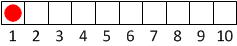
\includegraphics[width=2in]{test-amo2016-8-5a.png}
\end{center}
\end{uzdevums}


\begin{uzdevums}[AOPS.INT.8.5a]
Uz viena šķīvīša ir 7 zirņi, uz otra šķīvīša 9 zirņi. Ar vienu gājienu spēlētājs izvēlas 
kādu no šķīvīšiem un atņem no tā jebkuru skaitu zirņu (jāņem vismaz viens). Uzvar tas, kurš paņem 
pēdējo zirni. Kurš 
uzvar pareizi spēlējot - pirmais vai otrais spēlētājs?
\end{uzdevums}






\end{document}